% 首页信息自动生成

\section{数学符号测试}
绝对值:$\abs{x+y}$,范数:$\norm{\bm{v}}$

期望值:$\Ex{X}$, 条件期望:$\Ex[Y]{X}$

概率:$\Pr{A}$, 条件概率:$\Pr[B]{A}$

协方差:$\Cov{X}{Y}$, 方差:$\Var{X}$

极值点:$\argmin[x]{f(x)}$, $$\argmax[x]{g(x)}$$

长符号:$\longstack{~}{BCDEFGHIJKLM}$

\section{标记命令测试}
下划线:$\muline{abc}$,双下划线:$\muuline{def}$

%波浪线:$\muwave{ghi}$
删除线:$\msout{jkl}$

多重删除:$\mxout{mno}$,虚线:$\mdashuline{pqr}$

点线\footnote{\lipsum[2]}:$\mdotuline{stu}$

\section{图表测试}
\begin{figure}[H]
\centering
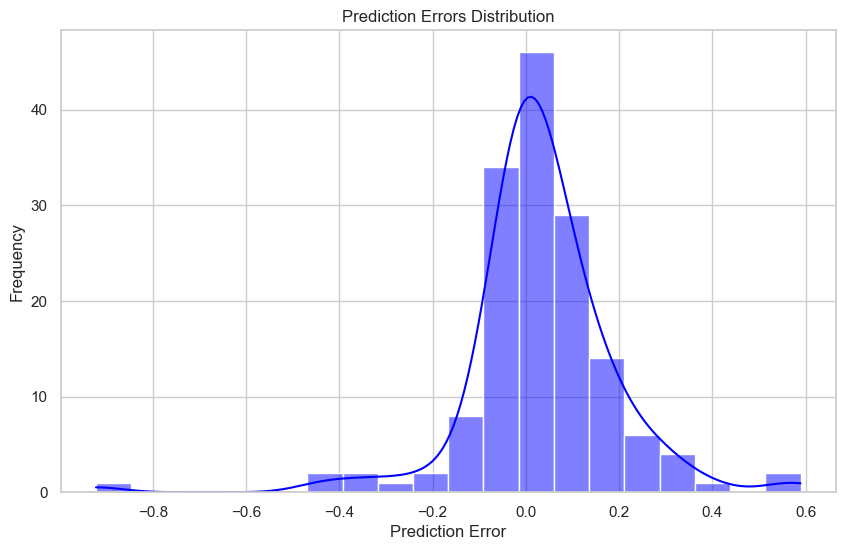
\includegraphics[width=0.3\textwidth]{test.png}
\caption{示例图片}
\label{fig:demo}
\end{figure}

如\figref{fig:demo}所示,\tabref{tab:demo}展示了数据。

\begin{table}[H]
\centering
\caption{示例表格}
\label{tab:demo}
\begin{tabular}{ll}
\toprule
项目 & 值 \\
\midrule
\subrow{一级条目} & 100 \\
\subrow{二级条目} & 200 \\
\bottomrule
\end{tabular}
\end{table}

\section{代码测试}
行内代码:\cmd{git commit -m "test"}

\begin{code}[caption=Python示例, language=Python, name=Python]
print("Hello World!")  # 简单输出
for i in range(10):
    !*\color{red}print(i)*!  # 带颜色逃逸
\end{code}

\section{题目环境测试}
\begin{prob}[难度系数]
这是一个多部分题目
\end{prob}
\begin{subsol}
\item 第一部分解:
\[ \int_0^1 x^2 dx = \frac{1}{3} \]
\item 第二部分解:
\begin{align*}
\Cov{X}{Y} &= \Ex{XY} - \Ex{X}\Ex{Y} \\
&= 0.5 - 0.2 \times 0.3 = 0.44
\end{align*}
\end{subsol}

\begin{prob}
证明勾股定理
\end{prob}
\begin{pf}
设直角三角形三边为$a,b,c$,则:
\[ a^2 + b^2 = c^2 \]
证毕。
\end{pf}

\section{化学式测试}
\chemfig{H_3C-[:30](-[:-90]OH)-[:-30]O-[:30]H} % 葡萄糖

\ce{CO2 + C -> 2 CO} % 化学反应式

\chemfig{*6((=O)-N(-CH_3)-(*5(=O)-N(-CH_3)-))} % 咖啡因

\ce{H2O} % 水分子

\chemfig{C(-[2]H)(-[6]H)(-[4]H)} % 甲烷

\ce{Zn^2+ + 2OH^- -> Zn(OH)2 v} % 沉淀反应

\chemfig{*6(=-N(-CH_3)-(*5(=O)-N(-CH_3)-))} % 尼古丁

\section{特殊功能测试}
分栏测试:\lipsum{5}

跨行超链接测试:\url{https://www.thisisaverylongurl.com/example/page?query=longurl}

\enteronecolumn
\section{临时单栏测试}
\lipsum{5}
\exitonecolumn

参考文献测试:引用文献\parencite{chen2016xgboost}
